
%

\exer{Surfing Porquerolles} 
\setcounter{ques}{0}

\begin{flushright}
\textit{D'après Concours Mines Ponts 2018.}
\end{flushright}
\begin{obj} ~\\
\begin{itemize}
\item Lire un fichier texte.
\item Analyser les données d'un fichiers. 
\end{itemize}
\end{obj}

\subsection*{Analyse vague par vague}

On considère ici que la mesure de houle est représentée par un signal $\eta(t) \in \mathbb{R}$, $t\in[0,T]$, avec
$\eta$ une fonction $C^1$.
On appelle niveau moyen $m$ la moyenne de $\eta(t)$ sur $[0, T]$.
On définit $Z_1$, $Z_2$, ..., $Z_n$ l’ensemble (supposé fini) des Passages par le Niveau moyen en Descente
(PND) (voir Figure suivante). À chaque PND, le signal traverse la valeur m en descente.
On suppose $\eta(0)>m$ et $\dfrac{\dd \eta }{\dd t}(0)>0$. On en déduit que $\eta(t)-m\geq 0$ sur $\left[0, Z_1\right]$.
Les hauteurs de vagues $H_i$ sont définies par les différences :
$$
 \left\{ 
\begin{array}{l}
H_1 = \max_{t\in[0,Z_1]} \eta(t)-\min_{t\in[Z_1,Z_2]} \eta(t) \\
H_i = \max_{t\in[Z_{i-1},Z_i]} \eta(t)-\min_{t\in[Z_{i-1},Z_{i+1}]} \eta(t) \\
\quad \quad \quad \text{pour }2\leq i <  n\\
\end{array}
\right.
$$

On définit les périodes de vagues par $T_i = Z_{i+1}-Z_i$.

\begin{center}
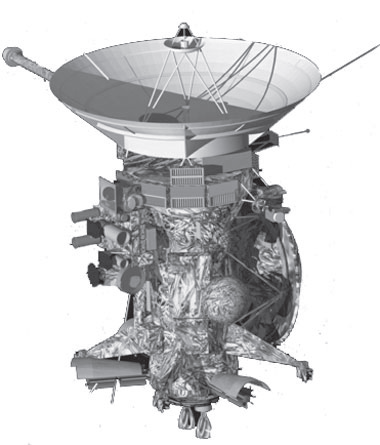
\includegraphics[width=\linewidth]{fig_00}
\end{center}

Le fichier \texttt{vagues.txt} contient un relevé des niveaux d'eau mesurés par une bouée au large de Porquerolles. (Pour ne pas se mentir, on a plutôt généré un profil qui pourrait vaguement ressembler à un tel relevé.)

Il est constitué de deux colonnes, séparées par une virgule, la première colonne correspondant à une mesure de temps (en secondes), la seconde colonne correspondant à une mesure de niveau de hauteur d'eau (en mètres). 

\question{Écrire une fonction \\ 
\texttt{lire\_fichier(file: str) -> list,list} 
prenant comme argument le nom d'un fichier et renvoyant la liste des temps que l'on notera \texttt{les\_t} et la liste des niveaux de vagues que l'on notera \texttt{liste\_niveaux}.}

\question{Écrire une fonction \\
\texttt{trace\_vagues(file: str) -> None} 
prenant comme argument le nom d'un fichier affichant le profil des vagues en fonction du temps.}

%Le résultat attendu est le suivant :  ......

\question{Écrire une fonction  \\
\texttt{moyenne(liste\_niveaux: list) -> float} 
prenant comme argument une liste non vide \texttt{liste\_niveaux}, et retournant sa valeur moyenne.}


\question{Écrire une fonction \\
\texttt{ind\_premier\_pzd(liste\_niveaux: list) -> int} 
retournant, s’il existe, l’indice
du premier élément de la liste tel que cet élément soit supérieur à la moyenne et l’élément suivant
soit inférieur à la moyenne. Cette fonction devra retourner $-1$ si aucun élément vérifiant cette condition n’existe.}

\question{Écrire une fonction \\
\texttt{ind\_dernier\_pzd(liste\_niveaux: list) -> int} 
 retournant l'indice $i$ du dernier élément de la liste tel que cet
élément soit supérieur à la moyenne et l’élément suivant soit inférieur à la moyenne. Cette fonction
devra retourner -2 si aucun élément vérifiant cette condition n’existe.}

On souhaite stocker dans une liste successeurs, les indices des points succédant (strictement)
aux PND (voir figure suivante).
\begin{center}
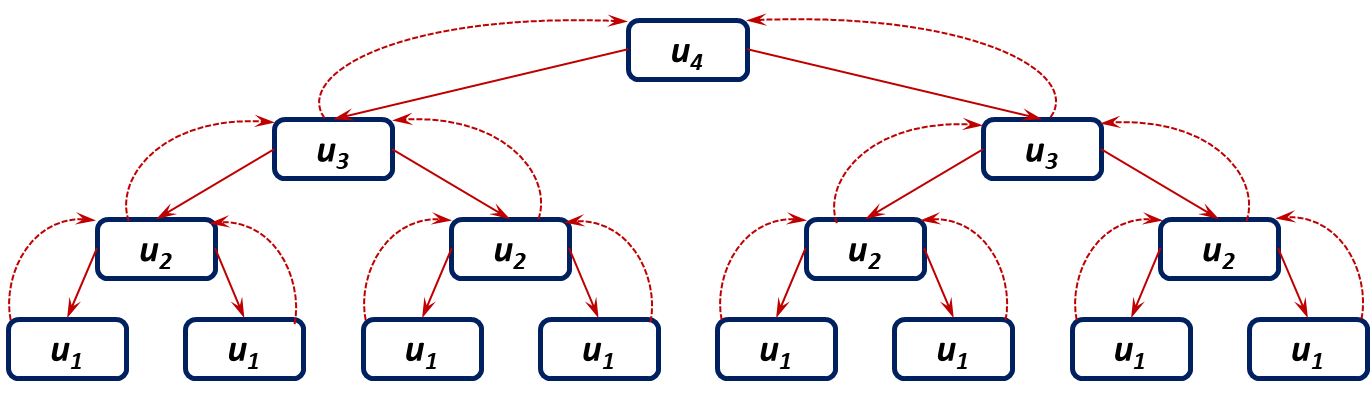
\includegraphics[width=\linewidth]{fig_01}
\end{center}

\question{Écrire une fonction  \\
\texttt{construction\_successeurs(liste\_niveaux: list) -> list} 
retournant la liste successeurs.}



\question{Écrire une fonction  \\
\texttt{decompose\_vagues(liste\_niveaux: list) -> list} 
qui permet de décomposer
une liste de niveaux en liste de vagues. On omettra les données précédant le premier PND et celles
succédant au dernier PND. Ainsi \texttt{decompose\_vagues([1, -1, -2, 2, -2, -1, 6, 4, -2, -5])}
(noter que cette liste est de moyenne nulle) retournera \texttt{[[-1, -2, 2], [-2, -1, 6, 4]]}.
}

On désire maintenant caractériser les vagues.
Ainsi, on cherche à concevoir une fonction \texttt{proprietes(liste\_niveaux: list) -> list} retournant une liste de
listes à deux éléments \texttt{[Hi,Ti]} permettant de caractériser chacune des vagues i par ses attributs :
\begin{itemize}
\item \texttt{Hi}, sa hauteur en mètres (m);
\item \texttt{Ti}, sa période en secondes (s).
\end{itemize}

\question{Écrire une fonction  \\
\texttt{proprietes(liste\_niveaux: list, dt:float) -> list}
réalisant cet objectif. \texttt{dt} représente la durée entre deux échantillons de la liste des temps obtenu à la question 2. On pourra utiliser les fonctions de Python \texttt{max(L)} et \texttt{min(L)} qui retournent le maximum et le minimum d’une
liste \texttt{L}, respectivement.}

\subsubsection*{Contrôle des données}
Plusieurs indicateurs sont couramment considérés pour définir l’état de la mer. Parmi eux, on
note :
\begin{itemize}
\item $H_{\text{max}}$ : la hauteur de la plus grande vague observée sur l’intervalle d’enregistrement $[0, T]$ ;
\item $H_{1/3}$ : la valeur moyenne des hauteurs du tiers supérieur des plus grandes vagues observées
sur $[0, T]$ ;
\item $T_{H1/3}$ : la valeur moyenne des périodes du tiers supérieur des plus grandes vagues observées
sur $[0, T]$.
\end{itemize}

\question{Écrire une fonction  \\
\texttt{H\_max(liste\_niveaux: list, dt: float) -> float}
prenant en argument la liste liste\_niveaux de la question 
renvoyant $H_{\text{max}}$.}

Afin de déterminer $H_{1/3}$ et $T_{H1/3}$, il est nécessaire de trier la liste des propriétés des vagues. 




La distribution des hauteurs de vague (voir figure suivante) lors de l’analyse vague par vague est
réputée être gaussienne. On peut contrôler ceci par des tests de skewness (variable désignée par $S$)
et de kurtosis (variable désignée par $K$) définis ci-après. Ces deux tests permettent de quantifier
respectivement l’asymétrie et l’aplatissement de la distribution.

\begin{center}
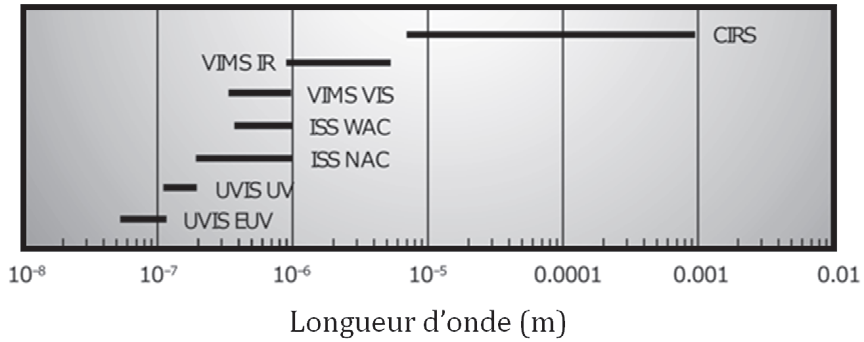
\includegraphics[width=\linewidth]{fig_02}
\end{center}


On appelle $\overline{H}$ et $\sigma^2$ les estimateurs non biaisés de l'espérance et de la variance, $n$ le nombre d'éléments $H_1$, $H_2$, ..., $H_n$.

On définit alors :

$$ S = \dfrac{n}{\left(n-1 \right)\left(n-2 \right)}\times \left( \dfrac{1}{\sigma^3}\right)\times \sum\limits_{i=1}^{n} \left(H_i - \overline{H} \right)^3
$$

$$ K = \dfrac{n}{\left(n-1 \right)\left(n-2 \right)\left(n-3 \right)}\times \left( \dfrac{1}{\sigma^4}\right)\times \sum\limits_{i=1}^{n} \left(H_i - \overline{H} \right)^4
-\dfrac{3\left(n-1 \right)^2}{\left(n-2 \right)\left(n-3 \right)}.
$$


Le test suivant est appliqué :
\begin{itemize}
\item si la valeur absolue de $S$ est supérieure à 0,3 alors l’horodate est déclaré non valide ;
\item si la valeur de $K$ est supérieure à 5 alors l’horodate est déclaré non valide.
\end{itemize}
On utilise la fonction \texttt{moyenne} pour estimer la valeur de $\overline{H}$. 
Même s'il serait aisé de coder la fonction écart type, on utilisera la fonction \texttt{
pstdev} de la bibliothèque \texttt{statistics} qui permet de retourner la valeur de l’écart type non biaisé $\sigma$.



\question{Écrire une fonction  \\
\texttt{skewness(liste\_niveaux) -> float} permettant de déterminer $S$.}